% Mathe Formelsammlung für HM2 SoSe 2011
% 2 Seiten
% Copyrightrechte des Quellcodes besitzt www.latex4ei.de


% Dokumenteinstellungen
% ======================================================================

% Dokumentklasse (Schriftgröße 6, DIN A4, Artikel)
\documentclass[6pt,a4paper]{scrartcl}

% Zusätzliche Pakete laden
\usepackage[utf8]{inputenc}		% Zeichenkodierung: UTF-8 (für Umlaute)   
\usepackage[german]{babel}		% Deutsche Sprache
\usepackage{multicol}			% Spaltenpaket
\usepackage{amsmath}			% erlaubt mathematische Formeln
\usepackage{amssymb}			% Verschiedene Symbole
\usepackage{esint}				% erweiterte Integralsymbole 
\usepackage{booktabs}			% bessere Tabellenlinien
\usepackage{graphicx}			% Zum Bilder einfügen benötigt
\usepackage{color}				% Farbiger Text möglich
\usepackage{pbox}				% Intelligent parbox: \pbox{maximum width}{blabalbalb \\ blabal}
\usepackage{undertilde}			% Für Welle unterhlab von Matrixbuchstaben benötigt
\usepackage{accents}			% Für eigene Ableitungspunkte benötigt
\usepackage{scrtime}
\usepackage{supertabular}		% Für lange Tabellen mit Umbruch

% Seitenlayout und Ränder:
\usepackage{geometry}
\geometry{a4paper,landscape, left=6mm,right=6mm, top=-1mm, bottom=3mm,includeheadfoot} 
\setlength{\parindent}{0mm}


% Dokumentbeschreibung
\title{Formelsammlung Höhere Mathematik 2 für EI}
\author{Emanuel Regnath}


% Kopf- und Fußzeile
% ======================================================================
\usepackage{fancyhdr}
\pagestyle{fancy}
\fancyhf{}
   \fancyfoot[C]{von Emanuel Regnath (Emanuel.Regnath@tum.de), Martin Zellner (martin.zellner@mytum.de) und Alexander Preißner (alexander.preissner@tum.de) - \copyright 2011 - 2012}
   \renewcommand{\headrulewidth}{0.0pt} %obere Linie ausblenden
   \renewcommand{\footrulewidth}{0.1pt} %obere Linie ausblenden

   \fancyfoot[R]{Stand: \todayV \ um \thistime \ Uhr \qquad \thepage}
   \fancyfoot[L]{Homepage: www.latex4ei.de -  Fehler bitte \emph{sofort} melden.}
% ----------------------------------------------------------------------




% Eigene Befehle und Befehlsüberschreibungen
% ======================================================================

% Schriftart SANS für bessere Lesbarkeit bei kleiner Schrift
\renewcommand{\familydefault}{\sfdefault} 
% Array- und Tabellenabstände vergrößern
\renewcommand{\arraystretch}{1.2}

% Befehle sichern
\let\oldvec = \vec
\let\olddot = \dot

% Eigene Befehle
\newcommand{\todayV}{\the\day.\the\month.\the\year}                          %%D.M.YYYY

\newcommand{\iset}[2]{\ensuremath{\bigl\{ \bigl. #1 \, \bigr| \, #2 \bigr\}}}					% intensional set
\newcommand{\eset}[1]{\ensuremath{\bigl\{#1\bigr\}}}											% extensional set
\newcommand{\enbrace}[1]{\ensuremath{\bigl\(#1\bigr\)}}											% extensional set
\newcommand{\norm}[1]{\ensuremath{\|#1\|}}														% Norm
\newcommand{\mat}[1]{\ensuremath{\begin{bmatrix} #1 \end{bmatrix}}}								% Matrix
\newcommand{\ma}[1]{\ensuremath{\utilde{\boldsymbol {#1}}}}										% Matrixsymbol
\newcommand{\vect}[1]{\ensuremath{\begin{pmatrix} #1 \end{pmatrix}}}							% Vektor
\newcommand{\mvect}[1]{\ensuremath{\left. \begin{matrix} #1 \end{matrix}  \right]}} 			% Matrixvektornotation
\newcommand{\gk}[1]{\ensuremath{\left\lfloor#1\right\rfloor}} 									% Gaußklammer
\newcommand{\sprod}[2]{\ensuremath{\left\langle #1, #2 \right\rangle }}							% Skalarprodukt
\newcommand{\abs}[1]{\ensuremath{\left\vert#1\right\vert}} 										% Betrag
\newcommand{\bdot}{\ensuremath{\boldsymbol \cdot}} 												% Dicker Punkt für Skalarprodukt
\newcommand{\svdots}{\ensuremath{\olddot :}}													% small vertical dots


% Überschreibungen
\renewcommand{\vec}[1]{\ensuremath{\underline{\boldsymbol {#1}}}}								% Vektor fett und unterstrichen
\renewcommand{\emph}[1]{\textbf{#1}}															% Hervorhebungen fett
\renewcommand*{\dot}[1]{\accentset{\mbox{\textrm{\large\bfseries .}} }{#1}}						% Dicker Ableitungspunkt
\renewcommand*{\ddot}[1]{\accentset{\mbox{\textrm{\large\bfseries .\hspace{-0.25ex}.}}}{#1}}	% Dicker Doppelableitungspunkt

% Abkürzungen
\newcommand{\ul}[1]{\ensuremath{\underline{#1}}}								% Untersteichen
\newcommand{\ol}[1]{\ensuremath{\overline{#1}}}									% Überstreichen
\newcommand{\Ra}[0]{\ensuremath{\Rightarrow}}									% Rightarrow
\newcommand{\ra}[0]{\ensuremath{\rightarrow}} 									% Rightarrow
\newcommand{\bs}[1]{\ensuremath{\boldsymbol{#1}}}								% Fett und kursiv im mathmode
\newcommand{\diff}{\ensuremath{\;\mathrm d}}									% differentielles delta
\newcommand{\grad}{\ensuremath{\mathrm{grad}\ }}								% Gradient
\renewcommand{\div}{\ensuremath{\mathrm{div}\ }}								% Divergenz
\newcommand{\rot}{\ensuremath{\mathrm{rot}\ }}									% Rotation
\newcommand{\Sp}{\ensuremath{\mathrm{Sp}\ }}									% Spur
\renewcommand{\i}{\ensuremath{\mathrm{i}}}										% Imaginäre Einheit
	% Für Mengen
	\newcommand{\N}{\ensuremath{\mathbb N}}
	\newcommand{\R}{\ensuremath{\mathbb R}}
	\newcommand{\C}{\ensuremath{\mathbb C}}




% Dokumentbeginn
% ======================================================================
\begin{document}


% Aufteilung in Spalten
\begin{multicols}{4}
	\parbox{2.3cm}{
		
\includegraphics[height=1.5cm]{./img/Logo.pdf}
	}
	\parbox{4cm}{
		\emph{\Large{Höhere Mathematik 2}}
	}
\vspace{-2mm} % Man muss optimieren wos nur geht ;)
% -------------------------------------------
% | 		Mathematik 2					|
% ~~~~~~~~~~~~~~~~~~~~~~~~~~~~~~~~~~~~~~~~~~~
%=======================================================================

\section{Nützliches Wissen $e^{\i x} = \cos (x) + \i \cdot \sin(x)$}
\subsection{Trigonometrische Funktionen}
\subsubsection{sinh, cosh \quad $\cosh^2(x)  \bs - \sinh^2(x) = 1$}
$\sinh x = \frac{1}{2}(e^x -e^{-x}) \qquad \quad \operatorname{arsinh}\ x:= \ln\left(x+\sqrt{x^2+1}\right) \\
\cosh x  = \frac{1}{2}(e^x +e^{-x}) \qquad \quad \operatorname{arcosh}\ x:= \ln\left(x+\sqrt{x^2-1}\right)\\
$\\
\begin{tabular}{ll}
	Additionstheoreme &	Stammfunktionen \\
	$\cosh x \,\; + \sinh x \,\,= e^{x}$ & $\int \sinh x \, dx = \cosh x + C$\\
	$\sinh({\rm arcosh}(x)) = \sqrt{x^2 - 1}$ & $\int \cosh x \, dx = \sinh x + C $\\
	$\cosh({\rm arsinh}(x)) = \sqrt{x^2 + 1}$ \\
\end{tabular}
%Kugel: $V_K = \frac{4}{3} \pi r^3$ \qquad $A_K = 4 \pi r^2$
%\subsection{subsection name} % (fold)
%\label{sub:subsection name|\(.)|(\w+)|([^\w\]+)/(?4:_:\L$1$2$3)/g}}

% subsection |\(.)|(\w+)|([^\w\]+)/(?4:_:\L$1$2$3)/g (end)

\subsubsection{sin, cos \quad $\sin^2(x) \bs + \cos^2(x) = 1$}
$\begin{array}{c|c|c|c|c|c|c|c|c}
x & 0 & \pi / 6 & \pi / 4 & \pi / 3 & \pi / 2 & \pi & \frac{3}{2}\pi & 2 \pi \\ \hline
\sin & 0 & \frac{1}{2} & \frac{1}{\sqrt{2}} & \frac{\sqrt 3}{2} & 1 & 0 & -1 & 0 \\
\cos & 1 & \frac{\sqrt 3}{2} & \frac{1}{\sqrt 2} & \frac{1}{2} & 0 & -1 & 0 & 1 \\     
\tan & 0 & \frac{\sqrt{3}}{3}&	1				 &	\sqrt{3} & \infty & 0 & - \infty & 0\\
\end{array}$ 
\begin{tabular}{l  l} 
	Additionstheoreme &  Stammfunktionen\\
 	$\cos (x - \frac{\pi}{2}) = \sin x$ & $\int x \cos(x) \diff x = \cos(x) + x \sin(x)$\\
 	
 	 $\sin (x + \frac{\pi}{2}) = \cos x$ & $\int x \sin(x) \diff x = \sin(x) - x \cos(x)$\\
 	
 	$\sin 2x = 2 \sin x \cos x $  & $\int \sin^2(x) \diff x = \frac12 \bigl(x - \sin(x)\cos(x) \bigr)$\\
     
 	$\cos 2x = 2\cos^2 x - 1$  & $\int \cos^2(x) \diff x = \frac12 \bigl(x + \sin(x)\cos(x) \bigr)$\\

 	$\sin(x) = \tan(x)\cos(x)$ & $\int \cos(x)\sin(x) = -\frac12 \cos^2(x)$ \\
\end{tabular}

\subsection{log \quad $\log(1) = 0$}
$a^x = e^{x \ln a} \qquad \quad \log_a x = \frac{\ln x}{\ln a} \qquad \quad \ln x \le x -1$

\subsection{Integrale:}
\begin{itemize}\itemsep-1pt
\item Partielle Integration: $\int uv'=uv-\int u'v$
\item Substitution: $\int f(\underbrace {g(x)}_{t}) \underbrace {g'(x)\,\mathrm dx}_{\mathrm dt}=\int f(t)\, \mathrm dt$
\end{itemize}

\everymath{\displaystyle}	% Formeln ab hier groß Schreiben
\begin{displaymath}\renewcommand{\arraystretch}{1.6}
\begin{array}{c|c|c}
F(x) & f(x) & f'(x) \\ \hline
\frac{1}{q+1}x^{q+1} & x^q & qx^{q-1} \\
\frac{2\sqrt{x^3}}{3} & \sqrt{x} & \frac{1}{2\sqrt{x}} \\
x\ln(x) -x & \ln(x) & \textstyle \frac{1}{x} \\
e^x & e^x & e^x \\
\frac{a^x}{\ln(a)} & a^x & a^x \ln(a) \\
-\cos(x) & \sin(x) & \cos(x) \\
-\ln |\cos(x)| & \tan(x) & \frac{1}{\cos^2(x)} \\
\ln |\sin(x)| & \cot(x) & \frac{-1}{\sin^2(x)} \\
x\arcsin (x)+\sqrt{1-x^2} & \arcsin(x) & \frac{1}{\sqrt{1-x^2}} \\
x\arccos (x)-\sqrt{1-x^2} & \arccos(x) & -\frac{1}{\sqrt{1-x^2}} \\
x\arctan (x)-\frac{1}{2} \ln \left| 1+ x^2 \right| & \arctan(x) & \frac{1}{1+x^2} \\
e^{(x)} (x-1) & x \cdot e^{(x)} & e^x(x+1) \\
\frac{1}{2} \Bigl(\sqrt{x^2 + 1} x + \sinh^{-1} (x)\Bigr) & \sqrt{1+x^2} & \frac{x}{\sqrt{x^2+1}}
\end{array}
\end{displaymath}
\everymath{\textstyle}

% Bitte keine Leichen im Quellcode stehen lassen...
%\begin{tabular}{c | c} 
% &  \\ \midrule
%\end{tabular}
\subsection{Determinante von $A\in \mathbb K^{n\times n}$: $\det(A)=|A|$}

 $\det\begin{pmatrix}A&0\\C&D\end{pmatrix}=\det\begin{pmatrix}A&B\\0&D\end{pmatrix}=\det(A)\cdot\det(D)$ \\
Hat $\ma A$ 2 linear abhäng. Zeilen/Spalten $\Rightarrow |A|=0$ \\
Entwicklung. n. $i$ter Zeile: $|A|=\sum\limits_{i=1}^n (-1)^{i+j} \cdot a_{ij} \cdot |A_{ij}|$ \qquad 


\subsection{Reihen}

$\underset{\text{Harmonische Reihe}}{\sum\limits_{n=1}^\infty \frac{1}{n} \ra \infty} \qquad   \underset{\text{Geometrische Reihe}}{\sum\limits_{n=0}^\infty q^n \stackrel{|q|<1}= \frac{1}{1-q}}  \qquad \underset{\text{Exponentialreihe}}{\sum\limits_{n = 0}^{\infty} \frac{z^n}{n!} = e^z}$


\section{Normen}
%===========================================================================================================================================================
Ist $V$ ein $\mathbb R$-VR, so ist $\| .\|: V \rightarrow \mathbb R, v \mapsto \|v\|$ eine Norm, falls
\begin{itemize}\itemsep0pt
	\item Definitheit: $\norm v \ge 0$ und $\norm v = 0 \Leftrightarrow v = 0$
	\item Homogenität: $\norm{\lambda v} = | \lambda | \cdot \norm v \quad \forall v \in V, \forall \lambda \in \mathbb R$
	\item Dreiecks-Ungleichung: $\norm{ v + w } \le \norm v + \norm w$	
\end{itemize}
%Falls eine Vektornorm $\norm{.}_V$ existiert, ist $(V, \norm{.})$ ein normierter Raum.

	\subsection{$l^p$-Normen für $v \in \mathbb K^n$}
	\begin{description}\itemsep-1pt
		\item[$p=1$ Betragsnorm:]  $\|v\|_1 = |v_1| + |v_2| + \ldots + |v_n|$
		\item[$p=2$ Euklidische Norm:] $\|v\|_2 = \sqrt{ v_1^2 + v_2^2 + \ldots + v_n^2}$
		\item[$p\rightarrow \infty$ Maximumsnorm:] $\|v\|_\infty = \max \iset{|v_i|}{i \in \{1,\ldots,n\}}$
	\end{description}
	
	\subsection{Matrixnormen für $A \in \mathbb K^{n\times n}$}
	Man nennt eine Matrixnorm $\norm{.}$ des $\mathbb K^{n \times n}$
	\begin{itemize} \itemsep0pt
		\item \textbf{submultiplikativ}, falls $\norm{AB} \le \norm{A} \cdot \norm{B} \quad \forall A,B \in \mathbb K^{n\times n}$
		\item \textbf{verträglich} mit einer Vektornorm $\norm{.}_V$ des $\mathbb K^n$, falls 
			\begin{equation*}
					\norm{A v}_V \le \norm A \cdot \norm {v}_V \quad \forall v \in \mathbb K^n, \forall A \in \mathbb K^{n \times n} 
			\end{equation*}
		\item \textbf{natürlich} bzw. \textbf{induziert} durch eine Vektornorm $\norm{.}_V$ des $\mathbb K^n$, falls
			\begin{equation*}
				\norm{A} := \sup \frac{\norm{Av}_V}{\norm{v}_V} \qquad V \in \mathbb K^n \setminus \{0\} \qquad \norm{E_n}=1
			\end{equation*}
	\end{itemize}
	
	\begin{description}\itemsep-1pt
		\item[Frobeniusnorm:] $\norm{A}_F = \sqrt{\sum_{j=1}^{n} \sum_{i=1}^{n} a_{ij}^2}$
		\item[Zeilensummennorm] $\norm{A}_{(\infty)} = \underset{i}{\max} \sum\limits_{j=1}^n |a_{ij}|$
		\item[Spaltensummennorm:] $\norm{A}_{(1)} = \underset{j}{\max} \sum\limits_{i=1}^n |a_{ij}| $	
		\item[Spektralnorm:] $\norm{A}_{(2)} = \sqrt{\lambda_{max} (A^\top \cdot A)}$
	\end{description}






		

\section{Taylor-Entwicklung}
%===========================================================================================================================================================
Man approximiert eine $m$-mal diffbare Funktion $f:I=[a,b] \rightarrow \mathbb R$ \\ in $x_0 \in I$ mit dem $m$-ten Taylorpolynom:\\
\boxed{ \ T_{m,f,x_0}(x)= \sum_{i=0}^{m} \frac{f^{(i)}(x_0)}{i!}(x-x_0)^i \ }\\
%\boxed{ T_{m,f,x_0}(x)=f(x_0)+\frac{f'(x_0)}{1!}(x-x_0)+\frac{f''(x_0)}{2!}(x-x_0)^2+\dotsc +\frac{f^{(m)}(x_0)}{m!}(x-x_0)^m }\\
Taylor-Entw. von Polynomen/Potenzreihen sind die Funktionen selbst.\\
Für $m \ra \infty$: Taylorreihe. \\
Konvergenzradius: $R = \underset{n\rightarrow \infty}{\lim} \abs{\frac{a_n}{a_{n+1}}}=\lim\limits_{n\rightarrow \infty}\frac{1}{\sqrt[n]{\abs{a_n}}}$

	\subsection{Das Restglied - die Taylorformel}
	Für $(m+1)$-mal stetig diffbare Funktionen gilt $\forall x \in I:$\\
	\boxed{ R_{m+1}(x) := f(x)- T_{m,f,x_0}(x) } $=$ \\
	$= \frac{1}{m!} \int_{x_0}^{x}(x-t)^m f^{(m+1)}(t)\mathrm dt$ \ \  (Integraldarst.)\\
	$= \frac{f^{(m+1)}(\xi)}{(m+1)!}(x-x_0)^{m+1}$ \quad
	$\xi \in [x, x_0]$ (Lagrange ) zur Berechnung der Genauigkeit\\
	
	\subsection{Landau-Notation}
	\begin{itemize}\itemsep-1pt
		\item $f(x) = o(g(x))$ für $x \rightarrow a \Leftrightarrow \lim\limits_{x \rightarrow a} \frac{f(x)}{g(x)} = 0$
		\item $f(x) = O(g(x))$ für $x \rightarrow a \Leftrightarrow |f(x)| \leq C|g(x)|$ für $x \in (a - \epsilon, a + \epsilon)$ u. $C > 0$\\ oder $0 \leq \limsup\limits_{x \rightarrow a} \abs{\frac{f(x)}{g(x)}} < \infty$
	\end{itemize}
	Bei \emph{Taylor-Entwicklung}:
	\begin{itemize}\itemsep-1pt
		\item $R_{m+1,f,x_0}(h) = f(x_0 + h) - T_{m,f,x_0}(h) = o(h^m)$\\ f muss m-mal differenzierbar sein
		\item $R_{m+1,f,x_0}(h) = f(x_0 + h) - T_{m,f,x_0}(h) = O(h^{m+1})$\\ f muss $(m+1)$-mal differenzierbar sein
	\end{itemize}
	\subsubsection{Rechenregeln}
	\begin{itemize}\itemsep-1pt
		\item $f = O(f)$
		\item $f = o(g) \quad\Rightarrow\quad f = O(g)$
		\item $f_1 = o(g)$ u. $f_2 = o(g) \quad\Rightarrow\quad f_1 + f_2 = o(g)$
		\item $f_1 = O(g)$ u. $f_2 = O(g) \quad\Rightarrow\quad f_1 + f_2 = O(g)$
		\item $f_1 = O(g)$ u. $f_2 = O(g) \quad\Rightarrow\quad f_1 \cdot f_2 = O(g_1 \cdot g_2)$
		\item $f_1 = O(g)$ u. $f_2 = o(g) \quad\Rightarrow\quad f_1 \cdot f_2 = o(g_1 \cdot g_2)$
	\end{itemize}
	\subsubsection{Elementarfunktionen}
	\begin{itemize}\itemsep-1pt
		\item Exponentialfunktion\\
		$e^x = \sum\limits_{k = 0}^m\frac{x^k}{k!} + O(x^{m + 1})$
		\item Trigonometrische Funktionen\\
		$\sin{x} = \sum\limits_{k = 0}^m(-1)^k\frac{x^{2k + 1}}{(2k + 1)!} + O(x^{2m + 3})$\\
		$\cos{x} = \sum\limits_{k = 0}^m(-1)^k\frac{x^{2k}}{(2k)!} + O(x^{2m + 2})$
		\item Logarithmusfunktion\\
		$\ln{(1 + x)} = \sum\limits_{k = 1}^m\frac{(-1)^{k + 1}}{k}x^k + O(x^{m + 1})$
	\end{itemize}
	

%=======================================================%
%									Iterationsverfahren										%
%=======================================================%
\section{Iterationsverfahren}
Mit Iterationsverfahren werden Nullstellen bestimmt.
\subsection{Fixpunktiteration}
\begin{enumerate}
	\item $f(x) = 0$ auf Form $g(x) = x$ bringen
	\item Konvergenz zeigen (Banach'scher Fixpunktsatz)
	\begin{itemize}\itemsep-1pt
		\item $g : I = [a;b] \mapsto I$ ist differenzierbar
		\item $\abs{g'(x)} \leq L \quad\forall x \in I$ mit $ 0 \leq L < 1$
	\end{itemize}
	\item Nullstelle mit Folge $x_{n+1} = g(x_n)$ und Startwert $x_0$ annähern
\end{enumerate}
\underline{Abschätzungen:} (Nullstelle x*)
\begin{itemize}\itemsep-1pt
	\item $\abs{x_n - x^*} \leq L^n\abs{x_0 - x^*}$ 'a priori'
	\item $\abs{x_n - x^*} \leq \frac{L}{1 - L}\abs{x_n - x_{n-1}}$ 'a posteriori'
	\item $\abs{x_n - x^*} \leq L\abs{x_{n-1} - x^*} \ra$ Lineare Konvergenz
\end{itemize}
\subsection{Newton-Verfahren}
Quadratische Konvergenz: $\abs{x_n - x^*} \leq C\abs{x_{n-1} - x^*}^2$ mit $C > 0$\\
Formel: $\boxed{x_{n+1} = x_n - \frac{f(x_n)}{f'(x_n)}}$ mit Startwert $x_0$\\
\underline{Voraussetzungen:}
\begin{itemize}\itemsep-1pt
	\item $f:[a,b] \mapsto \R$ ist \textbf{2-mal} stetig differenzierbar
	\item $m := \min\limits_{a \leq x \leq b}{\abs{f'(x)}} > 0$ u. $M := \max\limits_{a \leq x \leq b}{\abs{f''(x)}}$
	\item Wenn $\abs{x_0 - x^*} \leq \frac{2m}{M} \Rightarrow$ Konvergenz gegen x*
\end{itemize}
\underline{Abschätzungen:}
\begin{itemize}\itemsep-1pt
	\item $\abs{x^* - x_n} \leq \frac{M}{2m}\abs{x^* - x_{n-1}}^2; n = 1, 2, \ldots$
\end{itemize}



\section{Kurven}
%===========================================================================================================================================================
Eine Kurve ist ein eindimensionales Objekt.\\
$ \vec \gamma:[a,b] \rightarrow \mathbb R^n, t \mapsto \begin{pmatrix} \gamma_1(t) \\ \svdots \\ \gamma_n(t) \end{pmatrix} \quad \text{(Funktionenvektor)} $
%Eigenschaften von Kurven:
\begin{itemize}\itemsep-2pt
	\item $\mathcal C^0$-Kurve: Positionsstetigkeit (geschlossene Kurve)
	\item $\mathcal C^1$-Kurve: Tangentialstetigkeit (stetig diffbar)
	\item $\mathcal C^2$-Kurve: Krümmungsstetigkeit (2 mal stetig diffbar)
	\item regulär, falls $\forall t \in [a,b]:\dot \gamma(t) \ne \vec 0$ (Keine Knicke)
\end{itemize}
Besondere Punkte von Kurven:
\begin{itemize}\itemsep-2pt
	\item Singulär, falls $\dot \gamma(t)=\vec 0$ (Knick)
	\item Doppel-punk, falls $\exists t_1,t_2:t_1 \ne t_2 \ \land \ \gamma(t_1)=\gamma(t_2)$
	\item Horizontaler Tangentenpunkt, falls $\dot \gamma_1(t) \ne 0 \ \land \ \dot \gamma_2(t)=0$
	\item Vertikaler Tangentenpunkt, falls $\dot \gamma_1(t) = 0 \ \land \ \dot \gamma_2(t) \ne 0$
\end{itemize}
\emph{Bogenlänge} einer Kurve: $L(\gamma) = \int_{a}^{b} \norm{\dot \gamma(t)} \mathrm dt$ \\


Umparametrisierung $\gamma$ nach Bogenlänge ($\tilde \gamma$):
\begin{itemize} \itemsep0pt
	\item Bogenlängenfunktion: $s(t) = \int\limits_a^t \norm{\dot \gamma(\tau)} \mathrm d\tau$\\
		$s: [a,b] \ra [0,L(\gamma)], t \mapsto s(t)$
	%\item Umkehrfunktion: $s^{-1}:[0,L(\gamma)] \rightarrow [a,b]$ (streng monoton wachsend)
	\item $\tilde \gamma(t)=\gamma \bigl(s^{-1}(t) \bigr)$ \qquad $\norm{\ \dot{\tilde \!\! \gamma \!}\; (t)}=1 \forall t$ % Hässlich wie die Nacht aber geht iwie nicht anders...
\end{itemize}
Tangenteneineitsvektor an $\gamma(t): T(t)=\frac{\dot \gamma(t)}{\norm{\dot \gamma(t)} }$\\
Krümmung von $\gamma$: $\kappa(t)= \norm{\frac{\mathrm d^2 \gamma}{\mathrm d s^2}} = \frac{\norm{\dot T(t)}}{s'(t)}$\\
\\
\textbf{Vereinfachung} für $n=2$: $\gamma:[a,b] \rightarrow \mathbb R^2, t \mapsto \bigl(x(t),y(t)\bigr)$ \\
\everymath{\displaystyle}	% Formeln ab hier groß Schreiben
\boxed{ L(\gamma) = \int_a^b \sqrt{\dot x^2 + \dot y^2}\; \mathrm dt$ \qquad $\tilde{\kappa}(t)=\frac{\dot x \ddot y - \ddot x \dot y}{(\dot x^2 + \dot y^2)^{\frac{3}{2}}} } \\
\everymath{\textstyle}


	% \subsection{Funktionen als Kurve}
	% Funktion $f$ als Kurve: $\gamma:[a,b] \rightarrow \mathbb R^2, t \mapsto \begin{pmatrix} t \\ f(t) \end{pmatrix}$\\
	% Länge von $f$: $L(\gamma) = \int_a^b \sqrt{1+f'(t)^2}\; \mathrm dt$ \qquad Krümmung von $f$: $\varkappa(t)=\frac{f''(t)}{\sqrt{(1+f'(t)^2)^3}}$\\







\section{Skalarfelder}
%===========================================================================================================================================================
Ein Skalarfeld ordnet jedem Vektor eines Vektorraums einen Wert zu.\\
$ f:D\subseteq \mathbb R^n \rightarrow \mathbb R, (x_1,\ldots ,x_n) \mapsto f(x_1,\ldots ,x_n) $
\parbox{5.5cm}{
Teilmengen von $\mathbb R^n$: $D = [a_1,b_1] \times ... \times [a_n,b_n]$\\
Offene Kugelmenge vom Radius $r$: $B_r(x_0)$\\
\emph{Topologische Begriffe} für $D \subseteq \mathbb R^n$ } \parbox{1.0cm}{ 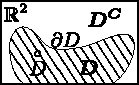
\includegraphics[height=0.8cm]{img/topologie.pdf} }
\begin{itemize}\itemsep-1pt
	\item Das Komplement $D^C$ von $D$: $D^C := \R^n \setminus D$
	\item innerer Punkt $x_0 \in \mathbb R^n$ des Inneren $\overset{\circ}{D}$ von $D$, falls \\
		$\exists \varepsilon > 0: B_\varepsilon (x_0) = \iset{x\in \mathbb R^n}{\norm{x-x_0} < \varepsilon} \subseteq D$
	\item Die Menge $D$ heißt offen, falls $D=\overset{\circ}{D}$
	\item Randpunkt $x_0 \in \mathbb R^n$ des Rands $\partial D$ von $D$, falls $\forall \varepsilon > 0:$ \\ 
		$B_\varepsilon(x_0) \cap D \ne \emptyset \ \land \ B_\varepsilon(x_0) \cap D^C \ne \emptyset \ \Rightarrow \ \partial D = \partial D^C$
	\item Abschluß $\ol D$ von $D$: $\overline{D}=D \cup \partial D$
	\item Die Menge $D$ ist abgeschlossen, falls $\partial D \subseteq D$
	\item beschränkt, falls $\exists \mu \in \mathbb R \forall x \in D: \norm{x} < \mu$
	\item kompakt, falls D abgeschlossen und beschränkt ist. 
\end{itemize}
Es gilt: Ist $D \subseteq \mathbb R^n$ offen, so ist $D^C$ abgeschlossen. \\
$\mathbb R$ und $\emptyset$ sind offen und abgeschlossen.




\subsection{Folgen, Grenzwerte, Stetigkeit im $\mathbb R^n$}
%-----------------------------------------------------------------------
Eine Folge $\bigl( X^{(k)} \bigr)$ ist eine Abbildung $\bigl(X^{(k)}\bigr):\mathbb N_0 \rightarrow \mathbb R^n, k\mapsto x^{(k)}$\\
Die Folge konvergiert, falls $\lim\limits_{k \rightarrow \infty} \norm{x-x^{(k)}} = 0$\\
Folge konvergiert, falls sie komponentenweise konvergiert!\\
\\
Für $f:D \subseteq \mathbb R^n \rightarrow \mathbb R$ bedeutet \\
Grenzwert: \quad  $\lim\limits_{x \rightarrow x_0} f(x) =c \Leftrightarrow f \bigl(X^{(k)} \rightarrow x_0 \bigr) \rightarrow c$\\
Stetigkeit: \quad \ $\forall x \in \mathbb R^n:\lim\limits_{x \rightarrow x_0} f(x) = f(x_0)$\\
Satz von Max. und Min.: Ist $f(\vec x)$ stetig und $D$ kompakt, so\\
% Ist $f:D \subseteq \mathbb R^n \rightarrow \mathbb R$ stetig und D kompakt, so\\
$\exists x_{max},x_{min} \in D \forall x\in D:f(x_{min}) \le f(x) \le f(x_{max})$





\subsection{Differentiation von Skalarfeldern - Gradient}
%-----------------------------------------------------------------------
% \boxed {f_{x_i}(x)=\lim\limits_{h \rightarrow 0} \frac{f(x+he_i)-f(x)}{h}}\\
$\nabla f(x) = \mathrm{grad} \bigl( f(x) \bigr) = \begin{pmatrix}  \frac{\partial}{\partial x_1} f(x) \\ \svdots \\ \frac{\partial}{\partial x_n} f(x) \end{pmatrix}$\\
\emph{Richtungsableitung:} \boxed { \partial_{\vec v} f(x) = \left\langle \nabla f(x), \vec v \right\rangle } \quad \boxed{ \norm{\vec v}=1 }\\
\\
\\
\textbf{Gradientenregeln:} $f,g:D \subseteq \mathbb R^n \rightarrow \mathbb R$ sind partiell diffbar:\\
Linearität: $\nabla(\lambda f + \mu g) (x) = \lambda \nabla f(x) + \mu \nabla g(x)$\\
Produkt: $\nabla (f \cdot g) (x) = g(x) \nabla f(x) + f(x) \nabla g(x)$\\
Quotient: $\nabla \Bigl( \frac{f}{g} \Bigr) = \frac{1}{g^2} \bigl( g(x)\nabla f(x) - f(x) \nabla g(x) \bigr)$\\
\\
Kettenregel\textbf{n:}\\
\begin{tabular}{l|l}
	$f:\mathbb R^n \rightarrow \mathbb R \land g:\mathbb R \rightarrow \mathbb R$ & $f:\mathbb R^n \rightarrow \mathbb R \land g:\mathbb R \rightarrow \mathbb R^n$\\ \midrule
	$h:= g \circ f: \mathbb R^n \rightarrow \mathbb R$	& $h:= f \circ g: \mathbb R \rightarrow \mathbb R$\\
	$\boxed{ \nabla h(x) = g'\big( f(x) \big) \cdot \nabla f(x)}$  &  $\boxed{h'(x)=\nabla f\big( g(x) \big)^T \cdot \dot g(t)}$
\end{tabular}

\subsection{Differentialoperatoren \qquad $\div(\rot(f)) = 0$}
\begin{tabular}{l|l}
	Operator & Definition \\ \midrule
	\pbox{2.0cm}{ Gradient: $\mathrm{grad}\; f$ \\ S-Feld $\rightarrow$ V-Feld } & $\nabla f = \vect{\frac{\partial f}{\partial x_1} \\ \svdots \\ \frac{\partial f}{\partial x_n} }$ \\ \midrule
	\pbox{2.0cm}{ Divergenz: $\mathrm{div}\; f$ \\ V-Feld $\rightarrow$ S-Feld } & ${\displaystyle \nabla^\top \bdot f = \sum\limits_{i=0}^n \frac{\partial f_i}{\partial x_i}}$\\ \midrule % \vect{\frac{\partial}{\partial x_1} \\ \svdots \\ \frac{\partial}{\partial x_n} }^\top \bdot \vect{ f_1 \\ \svdots \\ f_n }$ \\ \midrule
	\pbox{2.0cm}{ Rotation: $\mathrm{rot}\; f$ \\ V-Feld $\rightarrow$ V-Feld } & $\nabla \times f = \vect{\frac{\partial f_3}{\partial y}(x) - \frac{\partial f_2}{\partial z}(x) \\[2pt] \frac{\partial f_1}{\partial z}(x) -\frac{\partial f_3}{\partial x}(x) \\[2pt] \frac{\partial f_2}{\partial x}(x) -\frac{\partial f_1}{\partial y}(x) }$ \\ \midrule
	\pbox{2.0cm}{ Laplace: $\Delta\; f$ \\ S-Feld $\rightarrow$ S-Feld } & ${\displaystyle\underset{\nabla^\top \cdot (\nabla f)}{\nabla^2} = \sum \frac{\partial f}{\partial x_i x_i} }$ % \vect{\frac{\partial}{\partial x_1} \\ \svdots \\ \frac{\partial}{\partial x_n} }^\top \cdot \vect{\frac{\partial f}{\partial x_1} \\ \svdots \\ \frac{\partial f}{\partial x_n} }$ \\
\end{tabular}


\subsection{Höhere Partielle Ableitungen $\partial_j \partial_i f(x) = f_{x_i x_j} (x)$}
%-----------------------------------------------------------------------
$\mathcal C^m (D) = \eset{\text{m-mal stetig partiell diffbare Funktion auf D}}$\\
Satz von Schwarz: $f \in \mathcal C^2 (D) \Rightarrow f_{x_i x_j} (x)= f_{x_j x_i} (x) \quad \forall i,j$\\
\\
Mittelwertsatz ($f:D\subseteq \mathbb R^n \rightarrow \mathbb R, xy \in D \quad x,y \subseteq D$)\\
$\exists \xi \in \overline{x,y}$ mit $f(y)-f(x)=\nabla f^\top (\xi)(y-x)$\\
Es gilt $|f(y) - f(x)| \le c|y-x|$ mit $c= \mathrm{max} \norm{\nabla f(z)} \quad z \in \overline{x,y}$\\
\\
Hessematrix: $H_f (x) = \nabla^2 f(x) = \begin{bmatrix} \partial_{11} f(x)\ ...\ \partial_{1n} f(x) \\ \svdots \quad \qquad \qquad \svdots \\ \partial_{n1} f(x)\ ...\ \partial_{nn} f(x) \end{bmatrix}$\\
Die Hessematrix ist symmetrisch, falls $f \in \mathcal C^2(D)$\\
\\ 
\begin{tabular}{ll}
	$T_{2,f, \vec x_0} (\vec x) =$ $f(\vec x_0) +$ & (un inder rasant\footnote{Auch bekannt als der langsame Inder})\\
	\qquad $+ \nabla f(\vec x_0)^\top (\vec x-\vec x_0) +$ & (Tangentialebene)\\
	\qquad $+ \frac{1}{2}(\vec x-\vec x_0)^\top \ma H_f(x_0)(\vec x- \vec x_0)$ & (Schmiegequadrik)\\
	%\qquad $+ \qquad \svdots$ & (räumliche Matrix)\\
\end{tabular}

$T_{3,f,\vec a}(\vec x) = f(\vec a) + \sum \partial_i f(\vec a)(x_i - a_i) + \frac{1}{2} \sum \partial_i \partial_j f(\vec a)(x_i - a_i)(x_j - a_j) + \frac{1}{6} \sum \partial_i \partial_j \partial_k f(\vec a)(x_i - a_i)(x_j - a_j)(x_k - a_k)$

\subsection{Lineare Abbildungen}
%-----------------------------------------------------------------------
$f:V \rightarrow W$ heißt linear, falls

\begin{itemize}\itemsep0pt
	\item $f(v+w) = f(v) + f(w)$
	\item $f(\lambda v) = \lambda f(v)$
	\item Tipp: Prüfe ob $f(0) = 0$
\end{itemize}
Kern von $f$: $\ker (f) = \iset{v \in V}{f(v) = 0}$ ist UVR von $V$\\
Bild von $f$: $\mathrm{Bild}(f) = \iset{f(v)}{v \in V}$ ist UVR von $W$\\
\emph{Dualraum} $V^* = \iset{f:\mathbb R^n \rightarrow \mathbb R}{f=lin.}$\\
\emph{Injektiv} (aus $f(x) = f(y) \ra x = y)$), falls $\ker(f) = \eset{0}$ \\
\emph{Surjektiv} Alle Werte im Zielraum werden angenommen.

\subsubsection{Dimensionen}
\boxed{ \begin{array}{cc} \dim(V) = \dim \bigl(\ker(f) \bigr) + \dim \bigl(\mathrm{Bild}(f) \bigr) \\
\mathrm{rg}(f)=\dim\bigl( \mathrm{Bild}(f) \bigr) \end{array} }\\
Falls $\dim(V) = \dim(W)$, so gilt: \\
$f$ ist surjektiv $ \Leftrightarrow$ $f$ ist  injektiv $\Leftrightarrow$ $f$ ist  bijektiv. \\

\subsubsection{Die Darstellungsmatrix}
...beschreibt eine lineare Abbildung zwischem zwei endlichdimensionalen Vektorräumen.\\
\\
Sonderfälle: \\
$\ma{_{E_n} M(f)_{E_n}} = \ma{A}$ \quad $\|$ \quad
$\ma{_{E_n} M(id)_{B'}} = \ma B'$ \\ 
Koordinatenvektor $_B v$ von $v = \lambda_1 \vec b_1 + ... + \lambda_n \vec b_n $ bezüglich $\ma B$: \\
$_B v := \begin{pmatrix} \lambda_1 \\ \overset{:}: \\ \lambda_n \end{pmatrix} \in \mathbb K^n$\\


Darstellungsmatrix von $f$ bzgl.  der Basen $B$ in $C$ \\
$_C M(f)_B  = \begin{pmatrix}_C f(b_1)& _C f(b_2) &\ldots &_C	 f(b_n)\end{pmatrix} \in K^{m \times n}$
\\ \\
Darstellungsmatrizen bei Verkettungen von linearen Abbildungen
	$\underbrace{_D M (g \circ f)_B}_{r \times n} = \underbrace{_D M(g)_C}_{r \times m} \cdot \underbrace{_C M(f)_B}_{m \times n}$
	
\subsubsection{Die Bassistentransfomationsformel}

$f: \ma V \ra \ma W, \ma B, \ma B' \text{Basen von } \ma V \text{ in } \ma C, \ma C' \text{ Basen von } \ma W \text{ alle endlich }$
\boxed{	_{C'} M(f)_{B'} = _{C'} M(id)_C \cdot _C M(f)_B \cdot_B M(id)_{B'}}
\\
Bestimmung von $_{C'}M(id)_C$: LGS: $\bigl(C' | C\bigr) \overset{EZF}{\longrightarrow} \bigl( E_n | _{C'}M(id)_C \bigr)$
\\ \\
für $\ma V = \ma W = \ma K^n$ und $\ma C = \ma B = \ma E_n$ \\ \\
$f: \ma K^n \ra \ma K^n , f(v) = \ma A \vec v$
\\ \\
$ \ma{_{B'} M(f)_{B'}} = \ma{_{B'} M(id)_{E_n}} \cdot \ma{_{E_n} M(f)_{E_n}} \cdot \ma{_{E_n} M(id)_{B'}} =\\ \ma B'^{-1} \cdot \ma A \cdot \ma B' $


\subsection{Jacobimatrix = Fundamentalmatrix}
$\ma J_f (x) = \begin{bmatrix} \frac{\partial f_1}{\partial x_1} & ... & \frac{\partial f_1}{\partial x_n} \\ \svdots & & \svdots \\ \frac{\partial f_m}{\partial x_1} & ... & \frac{\partial f_m}{\partial x_n} \end{bmatrix} = \begin{pmatrix} \nabla f_1^\top \\ \svdots \\ \nabla f_m^\top \end{pmatrix}  \quad \in \mathbb R^{m \times n}$\\ \\
Rechenregeln für die Jacobimatrix:\\
$f,g: D \subseteq \mathbb R^n \rightarrow \mathbb R^m$ part. diffbar:\\
Linearität: $\ma J_{\alpha f + \beta g} = \alpha J_f + \beta J_g$\\
Produkt: $\ma J_{f^\top g} = g^\top J_f + f^\top J_g$ \quad $(\nabla f^\top g = J_f^\top g + J_g^\top f)$\\
Komposition: $\ma J_{g \circ f}(x) = \ma J_g\Bigl(f(x)\Bigr) \cdot \ma J_f(x)$\\
Umkehrfunktion: $\ma J_{f^-1} (f(x)) = \ma J_f (x)^{-1}$




\section{Koordinatensysteme}
%===========================================================================================================================================================
Um einen Vektor in anderen Koordinaten darzustellen:\\ \\
\begin{tabular}{c | c  l} 
&$\vect{ x & y & z}^\top$ &  \\ \midrule
Zylinder & $\begin{pmatrix} r \cdot \cos (\varphi) \\ r \cdot \sin (\varphi) \\ z \end{pmatrix}$ & $0 \le \varphi < 2 \pi$ \\ 
Kugel & $\begin{pmatrix} r \cdot \cos(\varphi) \sin(\theta) \\ r \cdot \sin(\varphi) \sin(\theta) \\ r \cdot \cos(\theta) \end{pmatrix}$ &$\begin{matrix}0 \le \theta \le \pi \\ 0 \le \varphi < 2 \pi\end{matrix}$
\end{tabular} \\ \\
 \\ 
% evtl. nochmal anschauen
\begin{tabular}{c | c} 
Zur Basistransformation: Transformationsmatrix $\ma S$ &  $f_{\text{kath}} =$ \\ \midrule
$\mat{ \cos(\varphi) &  -\sin(\varphi) & 0\\ \sin(\varphi) & \cos(\varphi) & 0 \\ 0 & 0 & 1 }$ &  $ \ma S_Z \cdot f_{\text{zyl}}$ \\
$\mat{ \cos(\varphi) \sin(\theta) & - \sin(\varphi) & \cos(\varphi)\cos(\theta) \\ \sin(\varphi)\sin(\theta) & \cos(\varphi) & \sin(\varphi)\cos(\theta) \\ \cos(\theta) & 0 & - \sin(\theta) }$ & $\ma S_k \cdot f_{\text{kugel}}$
\end{tabular}
\\ \\
Die Spalten entsprechen den orthonormalen Basisvektoren im jeweiligen Koordinatensystem. \\ $\Ra$ Trafo-Matrizen orthogonal: $\ma S^{-1} = \ma S^\top$\\


\begin{tabular}{c|l} 
 & Zylinderkoordinaten \\ \midrule
 $\nabla$ & $(\partial_r,\ \frac{1}{r}\partial_\varphi,\ \partial_z)^\top$ \\ \midrule
 $\div$ & $\frac{1}{r} \partial_r(r\cdot \vec f_r) + \frac{1}{r} \partial_\varphi(\vec f_\varphi) + \partial_z(\vec f_z)$ \\ \midrule
$ \Delta$ & $\frac{1}{r} \partial_{rr}(r\cdot f) + \frac{1}{r^2} \partial_{\varphi\varphi}f + \partial_{zz}f$
\end{tabular}
\\ \\ \\
\begin{tabular}{c|l} 
 & Kugelkoordinaten \\ \midrule

$\nabla$ & $(\partial_r,\ \frac{1}{r}\partial_\varphi,\ \frac{1}{r\sin\theta}\partial_\theta)^\top$\\ \midrule
$\div$ & $  \frac{1}{r^{2}}  \partial_r(r^2 \vec f_r) + \frac{1}{r \sin \theta} \partial_\varphi(\vec f_\varphi) + \frac{1}{r \sin \theta} \partial_\theta(\sin \theta \vec f_\theta)$\\ \midrule
$\Delta $ & $ \frac{1}{r^{2}} \partial_{rr}(r^2 f) + \frac{1}{r^2\sin^2\theta} \partial_{\varphi\varphi} (\sin\theta f) + \frac{1}{r^2\sin\theta} \partial_{\theta\theta} f$
\end{tabular}

\section{Implizite Funktionen $g$}
%===========================================================================================================================================================
... werden als Nullstellenmenge einer expl. Funktion $f$ angegeben.\\
$\iset{(x,y) \in \mathbb R^2 }{f(x,y) = 0}$ mit $y=g(x) \in \mathbb R$

\subsection{Satz über implizite Funktionen:}
Es gelte: $f: D \in \mathbb R^2 \ra \mathbb R$ \quad
$\ra $ implizite Gleichung $f(x,y) = 0$ \\
Bedinungen:
\begin{itemize} \itemsep0pt
	\item $D$ ist offen
	\item $f \in C^1 (D)$
	\item $\exists (x_0, y_0) \in D$ mit $f(x_0, y_0) = 0$
	\item $f_y(x_0, y_0) \not = 0$
\end{itemize}
\emph{$\Ra$} $ \exists I \subseteq \mathbb D: I = (x_0 - \epsilon, x_0 + \epsilon) , J \subseteq \mathbb R: J = (y_0 - \delta, y_0 + \delta)$ mit:
\begin{itemize}\itemsep0pt
	\item $I \times J \subseteq D$ in $f_y (x,y) \not = 0 \forall (x,y) \in I \times y$
	\item $\exists_1$ Funktion $g(x)$ mit $f(x,y) = 0$ ("$g$ wird implizit defniert")
	\item $g'(x) = \frac{-f_x(x, g(x))}{f_y (x, g(x))} = \frac{-f_x(x, y)}{f_y (x, y)} \quad \forall x \in I$ 
\end{itemize}

	
$g''(x) = - \frac{f_{xx} (x, g(x)) + 2f_{xy}(x,g(x)) \cdot g'(x) + f_{yy} (x, g(x)) \cdot (g'(x))^2}{f_y (x, g(x))} $

\subsection{Satz über implizite Funktionen (allgemein)}
$f: \mathbb R^{k+m} \ra \mathbb R^m$ stetig diffbar,\\ $z_0 = (x_0, y_0) \in \mathbb R^{k+m}$  	$x_0 \in \mathbb R^k, y_0 \in \mathbb R^m$ mit $f(z_0) = 0$
\\
Falls $J_{f,y} = (\frac{\partial f_{i(z_0)}}{\partial x_j})_{i = 1 \ldots m j= k +1 \ldots k+m}$ ist invertierbar $(\det J_{f,y} (z_0) \not = 0)$
\\
Dann: $\quad \exists$ offende Menge $I$ in $J$ mit $g: I \ra J$ mit $f(x,g(x)) = 0$ 


\subsection{Satz von der Umkehrabbildung}

$D \subseteq \mathbb R^n$ offen, $f: D \ra \mathbb R^n \in C^1 (D). X_0 \in D$ mit $J_f (x_0)$ ist invertierbar. \\
Dann: $\exists U$ Umgebung von $x_0$ mit $f |_U : U \ra f(U)$ ist bijektiv. \\
Die Umkehrfunktion $(f|_u)^{-1}$ ist stetig diffbar und es gilt: \\
$J(f|_U)^{-1} (f(x)) = (J_f (x))^{-1} \forall x \in U$


\subsection{Diagonalmatrix}

\underline{Bedingungen für Diagonalisierbarkeit:}
\begin{itemize} \itemsep0pt
	\item Das charakteristische Polynom $\chi_{A}$ zerfällt in Linearfaktoren\\
				$\chi_{A}(t) = (\lambda_1 - t)^{k_1}(\lambda_2 - t)^{k_2}\ldots(\lambda_r - t)^{k_r}$
	\item Die algebraischen Vielfachheiten der Eigenwerte stimmen mit den geometrischen überein\\
				$k_i = \dim V_{\lambda_i}$
	\item Jede \textbf{symmetrische} Matrix $A \in \R^{n \times n}$ ist diagonalisierbar
\end{itemize}

$\ma D = \begin{pmatrix} \lambda_1 & 0 & 0 \\ 0 & \lambda_2 & 0 \\ 0 & 0 & \lambda_3 \end{pmatrix}$ \qquad $\begin{array}{l} \ma D = \ma B^{-1} \ma A \ma B \\[0.5em] \ma B = \mat{\vec{EV}_1, \vec{EV}_2, ...} \end{array}$\\
$_B M(f)_B = _B M (id)_{E3} \cdot _{E3} M(f)_{E3} \cdot _{E3} M(id)_B$ \\
$B = ( _{E3} b_1 , _{E3} b_2 ,_{E3} b_3 ) = (v_1, v_2, v_3)$


\subsection{Definitheit}
Eine sym. Matrix $A = A^\top \in \mathbb R^{n\times n}$ heißt\\[0.3em]
$_{\text{\normalsize neg.}}^{\text{\normalsize pos.}}$ definit 
$ \Leftrightarrow$
$\forall v \in \mathbb R^n \setminus \eset{0} : \vec v^\top \ma A \vec v \gtrless 0$
$ \Leftrightarrow  $  Alle EW $\lambda \gtrless 0$\\
$_{\text{\normalsize neg.}}^{\text{\normalsize pos.}}$ semi definit $\ \Leftrightarrow\ $ $\forall v \in \mathbb R^n : \vec v^\top \ma A \vec v \gtreqless 0$ $\ \Leftrightarrow \ $  Alle EW $\lambda \gtreqless 0$\\
indefinit $\Leftrightarrow$
$\exists v,w \in \mathbb R^n: \vec v^\top
\ma A \vec v < 0 \ \land \ \vec w^\top \ma A \vec w > 0$ 
$\ \Leftrightarrow \ $  $\exists \lambda_1 > 0 \land \lambda_2 < 0$\\
Alle EW von $\ma A = \ma A^\top$ sind reel. $\lambda \in \mathbb R$ selbst wenn EV $v \in \mathbb C$!\\
Überprüfung mit $\det \ma A = \prod \lambda_i$ \qquad $\mathrm{Sp} \ma A = \sum \lambda_i$\\

\subsection{Eigenwerte, Eigenvektoren}
\emph{Eigenwerte:} $\det(\ma A - \lambda \ma 1) = 0$, Det-Entwickl., Polynom-Div. \\
$\Ra$ $\chi_A = (\lambda_1 - \chi)^{\nu_1} \cdot ... \cdot (\lambda_r - \chi)^{\nu_r}$ \quad $\nu_i = \mathrm{alg}(\lambda_i)$\\ \\
\emph{Eigenvektoren:} $\mathrm{Eig}_A (\lambda_i) = \ker(\ma A - \lambda_i \ma 1) = v_i$\\
$\ra \dim(\mathrm{Eig}_A (\lambda_i)) = \mathrm{geo}(\lambda_i)$ \quad $\forall i : 1 \le \mathrm{geo}(\lambda_i) \le \mathrm{alg}(\lambda_i)$\\ \\
\boxed{\ma A \vec v = \lambda \vec v} mit $\vec v$ EV von $\ma A$ \\
\underline{Ähnlichkeit von Matrizen:} Matrizen A und B sind ähnlich, wenn
\begin{itemize}
	\item sie die gleichen Eigenwerte besitzen
	\item die algebraischen mit den geometrischen Vielfachheiten der Eigenwerte übereinstimmen
	\item Es gilt: $\det A = \det B$
\end{itemize}

\subsection{Schnurzerlegung}
$\ma R = \ma U^T \ma A \ma U$\quad geht für jede quadratische Matrix $\ma A$, deren charakatristische Polynom in Linearfaktoren zerfällt.\\
$\ma U$ ist orthogonal $\ma U^\top = \ma U^{-1}$ \quad $\ma R$ ist obere Dreiecksmatrix

\begin{enumerate} \itemsep0pt
\item Finde 1 EW $\lambda_1$ und bestimme EV $\vec v_1$ zu $\lambda_1$ mit $\norm{\vec v_1} = 1$
\item Ergänze $\vec v_1$ zu einer ONB:\\ $\ma B_1 = (\vec v_1, \vec w_2, ..., \vec w_n,) \in \mathbb R^{n \times n} \qquad (\ma B^\top_1 = \ma B^{-1}_1)$\\
\item Berechne $_{B_1} \ma M(f)_{B_1} = \ma B^\top_1 \ma A \ma B_1 = \mat{\lambda_1 & * & * \\ 0 & \ma A_1 &  \\ 0 &  &  }$  \\ 
		Das liefert $\ma A_1 \in \mathbb R^{(n-1)\times(n-1)}$\\
\item Wiederhole 1. bis 4. mit $\ma A_1$ anstelle von $\ma A$, bis
\end{enumerate}
%\item $\tilde{\ma A_1} = _{B2} M(f)_B2 = \ma B_2^\top \ma A_1 \ma B_2 $
Abbruchbedingung: $\ma B_i$ ist $(2 \times 2)$-Matrix, dann berechne\\
$\ma U = \ma B_1 \cdot \mat{1  & 0 \\ 0 & \ma B_2 \\} \cdot \mat{1 & 0 & 0 \\ 0 & 1 & 0 \\ 0 & 0 & \ma B_3 \\} \cdot \ldots $\\
Und schließlich: $\ma R = \ma U^\top \ma A \ma U$ \quad $\Ra \ma R$ ist obere Dreiecksmatrix: Party!



\subsection{Singulärwertzerlegung \quad $\bs A=\bs U \bs\Sigma \bs V^\top$}
\begin{itemize}\itemsep0pt
\item Bestimme die Eigenwerte $\lambda_1, . . . , \lambda_n$ von $\ma A^\top \cdot \ma A$(sym.) aus $\R^{n \times n}$
und sortiere: \\
$\lambda_1 \ge \lambda_2 \ge \ldots \ge \lambda_n \ge 0$ \\
\item Bestimme dann eine ONB $\ma V = (v_1, . . . , v_n)$ aus EV
von $\ma A^\top \cdot \ma A $
\item  $\underset{m \times n}{\ma \Sigma} = \text{diag}(\sigma_1, \ldots, \sigma_2) $ mit $\boxed{\sigma_i = \sqrt{\lambda_i}}$ (Singulärwerte) \\
			(Ergänze mit Nullspalten/ Zeilen, dass $\dim \Sigma = \dim A$)
\item $\underset{m \times n}{\ma \Sigma}  = \underset{m \times m}{\ma U^\top} \cdot \underset{m \times n}{\ma A} \cdot \underset{n \times n}{\ma V}$ \quad ($\ma U, \ma V$ sind orthogonal)\\  % \text{ mit } \ma A \in \mathbb R^{m \times n}
\item Bestimme $\ma U=(\vec u_1, \vec u_2, \ldots \vec u_k)$ mit $k = \min \eset{m, n}$ \\
$\boxed{\vec u_i =\frac{1}{\sigma_i}\ma A \vec v_i}$ \\
Falls $n \le m$, ergänze die Vektoren $\vec u_i$ zu ONB $\ma U$ des $\R^n$.
\end{itemize}



\subsection{Extremwerte von Skalarfeldern $f(\vec x)$}
\subsubsection{Extremewerte ohne NB} % (fold)
\begin{itemize} \itemsep0pt
	\item Suche Kandidaten (stationäre Punkte): $\eset{\vec x_0}:{\nabla f(\vec x_0) = 0}$
	\item Falls $H_f(\vec x_0) \begin{cases} \text{neg. definit} & \Rightarrow \vec x_0 = \text{lok. Max.} \\ \text{pos. definit} & \Rightarrow \vec x_0 = \text{lok. Min.} \\ \text{indefinit} & \Rightarrow \vec x_0 = \text{Sattelpunkt} \\ \text{semidefinit} & \Rightarrow \vec x_0 = \text{keine Aussage} \end{cases}$\\
	\item globale Extreme $\ra $ prüfe Rand
\end{itemize}

% subsection subsection name (end)

\subsubsection{Lineare Ausgleichsrechnung}
Man betrachtet eine Funktion $b = f(t) = x_0 + x_1t + \ldots + x_nt^n$ mit unbekannten Koeffizienten $x_0, x_1, \ldots x_n$. Es sind m Paare $(b_i, t_i)$ gegeben und sucht
den Vektor $\vec x = (x_0, x_1, \ldots, x_n)^T$, für den $r_i(x) = b_i - x_0 - x_1t - \ldots - x_nt^n$ minimal sind. \\ \\
\underline{Aufgabe:} Minimiere $\sum\limits_{i = 1}^m (b_i - x_0 - x_1t - \ldots - x_nt^n)^2$ \\
$\Leftrightarrow$ Minimiere $\norm{\vec r(\vec x)}^2$ mit $\vec r(\vec x) = \vec b - \ma A \vec x$ \\
$\ma A = \mat{
	1 & t_1 & t_1^2 & \cdots & t_1^n \\
	1 & t_2 & t_2^2 & \cdots & t_2^n \\
	\vdots & \ddots & \ddots & \ddots & \vdots \\
	1 & t_m & t_m^2 & \cdots & t_m^n
}, \vec b = \vect{b_1 \\ b_2 \\ \svdots \\ b_m}$ \\
Man erhält Minimum durch Lösen der Normalengleichung \\
$\boxed{\ma A^T \ma A \vec x = \ma A^T \vec b}$

\subsubsection{Extremwerte von $f(\vec x)$ mit Nebenbedingung}
Es seien $f,g:\Omega \subset \R^n \mapsto \R$
\begin{itemize} \itemsep0pt
	\item NB $g(x) = 0$ ist nach einer Variable auflösbar. \\
	$\ra$ Setze $x_i$ in $f(x)$ ein $\ra$ Bestimme EW
	\item Lagrange-Funktion \\
	Nebenbedingung $g(x) = 0$\\
	$\boxed{L(x, \lambda) = f(x) + \lambda g(x)}$
	\begin{itemize} \itemsep0pt
		\item Regularitätsbedingung: \\
			$\nabla{g(x)} \neq 0 \quad \forall x \in \Omega$
		\item Kandidaten: \\
			$\nabla{L(x, \lambda)} = 0 \Ra \begin{cases}
				\begin{array}{r}
					\nabla{f(x)} + \lambda\nabla{g(x)} = 0 \\
					g(x) = 0
				\end{array}
			\end{cases}$
		\item Vergleiche die Funktionswerte der Kandidaten \\
			\ra Entscheidung über Extrema (auch Rand betrachten)
	%\item Kandidaten 1. Art \\
	%$\nabla g(x) = 0 $ \\
	%$g(x) = 0$ muss auch erfüllt sein
	%\item Kandidaten 2. Art: \\
	%$\nabla L (x, \lambda) = 0$
	%\item Vergleich der Funktionswerte der Kandidaten $ \ra$ Entscheide über Max/ Min bzw. betrachte Rand
	\end{itemize}
\end{itemize}
	PS: Lagrange bestiehlt kleine Kinder!!!!





\subsection{Sonstiges}



\subsection{Skalares Kurvenintegral}
von Skalarfeld $f(\vec x)$ entlang einer Kurve $\vec \gamma(t)$ mit $\vec x, \vec \gamma \in \mathbb R^n$\\
\boxed{ \int\limits_\gamma f \ \mathrm ds := \int\limits^b_a f\bigl(\vec \gamma(t)\bigr) \cdot \norm{\vec{\dot \gamma}(t)} \mathrm dt }\\
Im Fall $n = 2$ gibt $\int\limits_\gamma f \ \mathrm ds$ den Flächeninhalt unter $f$ entlang der Spur von $\vec \gamma$ an.
$L(\vec \gamma)$ ist das skalares Kurvenintegral über $f = 1$\\
Anmerkung: Ist $\varrho(x,y,z)$ die Masse- oder Ladungsdichte eines Drahtes so ist die Gesamtmasse $M$: \\
$\int\limits_\gamma f \ \mathrm ds = \int\limits^b_a \varrho \bigl(\vec \gamma(t)\bigr) \cdot \norm{\vec{\dot \gamma}(t)} \mathrm dt$\\
Der Schwerpunkt $\vec S = (S_1, S_2, S_3)$ ist:
$S_i = \frac{1}{M(\vec \gamma)} \cdot \int\limits_\gamma x_i \varrho \ \mathrm ds$
\subsection{vektorielles Kurvenintegral}
von einem Vektorfeld $\vec v(\vec x)$ längs der Kurve $\vec \gamma$ mit $\vec x, \vec v, \vec \gamma \in \mathbb R^n$\\
\boxed{ \int \vec v \bs \cdot \mathrm d\vec s := \int\limits^b_a \vec v \bigl(\vec \gamma(t)\bigr)^\top \bs \cdot \vec{\dot \gamma}(t) \ \mathrm dt }\\

Für beide Integrale gilt:\\
$\forall \lambda,\mu \in \mathbb R, \forall f,g$\\
$\int\limits_{\vec \gamma} \lambda f + \mu g \ \mathrm ds = \int\limits_{\vec \gamma} \lambda f \ \mathrm ds + \int\limits_{\vec \gamma} \mu g \ \mathrm ds$\\
Ist $\gamma = \sum \gamma_i$ so gilt: $\int\limits_{\vec \gamma} f \ \mathrm ds = \sum \int\limits_{\vec \gamma_i} f \ \mathrm ds$\\
$\int\limits_{\vec \gamma} f \ \mathrm ds = \underset{\text{Bei VF}}{(-)} \ \int\limits_{- \vec \gamma} f \ \mathrm ds$\\


$\ra g''(42) > 9000$ (over 9000)

\subsection{Integrabilitätsbedingung (Gradientenfeld)} % (fold)
$\Ra$ Kurve muss einfach zusammenhängend sein. \\
(Man muss die Kurve auf einen Punkt zusammenziehen könnnen) \\ \\
$f:D \subset \R^n \mapsto \R^n$ ist ein Gradientenfeld, wenn $f(x) = \nabla{F(x)}$ \\
$\Leftrightarrow \boxed{J_f(x) = J_f(x)^T}$ bzw. $\partial_{x_i}f_j(x) = \partial_{x_j}f_i(x)$ \\ \\
\underline{Sonderfälle:}
\begin{itemize} \itemsep0pt
	\item $n = 2$: $\frac{\partial v_1}{\partial y} = \frac{\partial v_2}{\partial x}$
	\item $n = 3$: $\rot v = 0 \Ra $ Integrabilitätsbedinung ist erfüllt.
\end{itemize}


\parbox{2.0cm}{
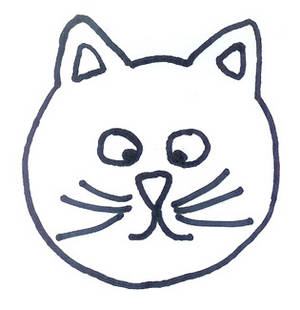
\includegraphics[height=0.8cm]{./img/cat.jpg}
}
\parbox{4.0cm}{
	Auch wichtig: Schrödingers Katze
}

% Ende der Spalten
\end{multicols}

% Dokumentende
% ======================================================================
\end{document}
